%===============================================================================
% LaTeX sjabloon voor de bachelorproef toegepaste informatica aan HOGENT
% Meer info op https://github.com/HoGentTIN/latex-hogent-report
%===============================================================================

\documentclass[dutch,dit,thesis]{hogentreport}

% - If necessary, replace the option `dit`' with your own department!
%   Valid entries are dbo, dbt, dgz, dit, dlo, dog, dsa, soa
% - If you write your thesis in English (remark: only possible after getting
%   explicit approval!), remove the option "dutch," or replace with "english".

\usepackage{lipsum} % For blind text, can be removed after adding actual content

%% Pictures to include in the text can be put in the graphics/ folder
\graphicspath{{../graphics/}}

%% For source code highlighting, requires pygments to be installed
%% Compile with the -shell-escape flag!
\usepackage[section]{minted}
%% If you compile with the make_thesis.{bat,sh} script, use the following
%% import instead:
%% \usepackage[section,outputdir=../output]{minted}
\usemintedstyle{solarized-light}
\definecolor{bg}{RGB}{253,246,227} %% Set the background color of the codeframe

%% Change this line to edit the line numbering style:
\renewcommand{\theFancyVerbLine}{\ttfamily\scriptsize\arabic{FancyVerbLine}}

%% Macro definition to load external java source files with \javacode{filename}:
\newmintedfile[javacode]{java}{
    bgcolor=bg,
    fontfamily=tt,
    linenos=true,
    numberblanklines=true,
    numbersep=5pt,
    gobble=0,
    framesep=2mm,
    funcnamehighlighting=true,
    tabsize=4,
    obeytabs=false,
    breaklines=true,
    mathescape=false
    samepage=false,
    showspaces=false,
    showtabs =false,
    texcl=false,
}

% Other packages not already included can be imported here

%%---------- Document metadata -------------------------------------------------
\author{Roy Barneveld}
\supervisor{J. Willem (HoGent, \href{mailto:jan.willem@hogent.be}{jan.willem@hogent.be})}
\cosupervisor{J. Willem (HoGent, \href{mailto:jan.willem@hogent.be}{jan.willem@hogent.be})}
\title{Ontwikkeling van een privacybewust spelling- en gram\-ma\-ti\-ca\-con\-tro\-le-toet\-sen\-bord voor Android met Rob\-BERT \\ en Ten\-sor\-Flow}
\academicyear{\advance\year by -1 \the\year--\advance\year by 1 \the\year}
\examperiod{1}
\degreesought{\IfLanguageName{dutch}{Professionele bachelor in de toegepaste informatica}{Bachelor of applied computer science}}
\partialthesis{false} %% To display 'in partial fulfilment'
%\institution{Internshipcompany BVBA.}

%% Add global exceptions to the hyphenation here
\hyphenation{back-slash}

%% The bibliography (style and settings are  found in hogentthesis.cls)
\addbibresource{bachproef.bib}            %% Bibliography file
\addbibresource{../voorstel/voorstel.bib} %% Bibliography research proposal
\defbibheading{bibempty}{}

%% Prevent empty pages for right-handed chapter starts in twoside mode
\renewcommand{\cleardoublepage}{\clearpage}

\renewcommand{\arraystretch}{1.2}

%% Content starts here.
\begin{document}

%---------- Front matter -------------------------------------------------------

\frontmatter

\hypersetup{pageanchor=false} %% Disable page numbering references
%% Render a Dutch outer title page if the main language is English
\IfLanguageName{english}{%
    %% If necessary, information can be changed here
    \degreesought{Professionele Bachelor toegepaste informatica}%
    \begin{otherlanguage}{dutch}%
       \maketitle%
    \end{otherlanguage}%
}{}

%% Generates title page content
\maketitle
\hypersetup{pageanchor=true}

%%=============================================================================
%% Voorwoord
%%=============================================================================

\chapter*{\IfLanguageName{dutch}{Woord vooraf}{Preface}}%
\label{ch:voorwoord}

%% Het voorwoord is het enige deel van de bachelorproef waar je vanuit je
%% eigen standpunt (``ik-vorm'') mag schrijven. Je kan hier bv. motiveren
%% waarom jij het onderwerp wil bespreken.
%% Vergeet ook niet te bedanken wie je geholpen/gesteund/... heeft

Het onderwerp van deze bachelorproef is mij toegewezen door mijn promotor en co-promotor, meneer Jan Willem. Zijn begeleiding en ondersteuning gedurende dit project zijn van onschatbare waarde geweest, en ik wil hem dan ook hartelijk bedanken. De snelle reacties op mijn vragen en zijn constante bijstand hebben me enorm geholpen om tot dit eindresultaat te komen. Zijn waardevolle adviezen hebben een belangrijke bijdrage geleverd aan mijn onderzoek.
\vspace{0.5cm}

Hoewel ik zelf nog geen echte ervaring had in het domein van artificiële intelligentie, heb ik altijd een grote interesse gehad in dit vakgebied. Deze bachelorproef bood mij een uitstekende kans om meer te leren over een onderwerp dat steeds belangrijker wordt in onze samenleving. De integratie van AI in verschillende aspecten van ons dagelijks leven benadrukt hoe cruciaal het is om hier kennis over te hebben.
\vspace{0.5cm}

Het unieke verloop van deze bachelorproef zorgde ervoor dat het soms een behoorlijke uitdaging was, wat leidde tot momenten van intensieve inspanning en soms een stroeve voortgang. Desondanks heeft deze ervaring me veel geleerd en mijn interesse in AI verder aangewakkerd.
\vspace{0.5cm}

Daarnaast wil ik ook Jordy Callant bedanken voor het nalezen van deze thesis en het geven van waardevol advies. Zijn feedback heeft geholpen om de kwaliteit van mijn werk te verbeteren.
\vspace{0.5cm}

Met dank aan allen die op enige wijze hebben bijgedragen, presenteer ik deze bachelorproef met trots en hoop ik dat het een bijdrage levert.

\vspace{2cm}
\begin{flushleft}
    Roy Barneveld \\
    Gent, 24 Mei 2024
\end{flushleft}
%%=============================================================================
%% Samenvatting
%%=============================================================================

% Een goede abstract biedt een kernachtig antwoord op volgende vragen:
%
% 1. Waarover gaat de bachelorproef?
% 2. Waarom heb je er over geschreven?
% 3. Hoe heb je het onderzoek uitgevoerd?
% 4. Wat waren de resultaten? Wat blijkt uit je onderzoek?
% 5. Wat betekenen je resultaten? Wat is de relevantie voor het werkveld?
%
% Daarom bestaat een abstract uit volgende componenten:
%
% - inleiding + kaderen thema
% - probleemstelling
% - (centrale) onderzoeksvraag
% - onderzoeksdoelstelling
% - methodologie
% - resultaten (beperk tot de belangrijkste, relevant voor de onderzoeksvraag)
% - conclusies, aanbevelingen, beperkingen
%
% LET OP! Een samenvatting is GEEN voorwoord!

%%---------- Nederlandse samenvatting -----------------------------------------
%
% TODO: Als je je bachelorproef in het Engels schrijft, moet je eerst een
% Nederlandse samenvatting invoegen. Haal daarvoor onderstaande code uit
% commentaar.
% Wie zijn bachelorproef in het Nederlands schrijft, kan dit negeren, de inhoud
% wordt niet in het document ingevoegd.

\IfLanguageName{english}{%
\selectlanguage{dutch}
\chapter*{Samenvatting}
\lipsum[1-4]
\selectlanguage{english}
}{}

%%---------- Samenvatting -----------------------------------------------------
% De samenvatting in de hoofdtaal van het document

\chapter*{\IfLanguageName{dutch}{Samenvatting}{Abstract}}

In deze scriptie wordt een privacybewust spelling- en grammaticacontrole-toet\-sen\-bord voor Android ontwikkeld, met gebruik van RobBERT en TensorFlow. Het centrale thema van dit onderzoek is de ontwikkeling van een toetsenbord dat nauwkeurige taalverwerking biedt en offline functioneert, zodat gebruikers volledige controle over hun persoonlijke gegevens behouden. De onderzoeksvraag richt zich op hoe een dergelijk toetsenbord kan worden ontwikkeld, met een focus op de ondersteuning van Nederlandse taal, de balans tussen nauwkeurigheid, privacy, en de schaalbaarheid naar andere talen en gebruikssituaties.
Het doel van dit onderzoek was een proof-of-concept te ontwikkelen voor een privacybewust toetsenbord, waarbij een geoptimaliseerde versie van het RobBERT-model wordt gebruikt voor offline taalverwerking. De verwachte resultaten omvatten een werkend prototype dat nauwkeurige spelling- en grammaticacontrole biedt zonder externe gegevensverwerking, volledige controle van de gebruiker over persoonlijke gegevens, flexibiliteit voor uitbreiding naar meerdere talen, en inzichten in de balans tussen nauwkeurigheid en privacy in taalverwerkingsmodellen.
De methodologie van dit onderzoek omvat verschillende fasen: een uitgebreide literatuurstudie naar bestaande NLP-technologieën en privacykwesties, de selectie van geschikte taalmodellen waarbij uiteindelijk gekozen is voor RobBERT 2023-dutch-large vanwege zijn prestaties in Nederlandse taaltaken, de conversie van dit model vanuit PyTorch naar TensorFlow Lite, geschikt voor mobiele apparaten, en de integratie van dit model in een bestaande open-source toetsenbord applicatie.
De resultaten van het onderzoek tonen aan dat het mogelijk is een werkend prototype te ontwikkelen dat nauwkeurige spelling- en grammaticacontrole biedt zonder externe gegevensverwerking, wat bijdraagt aan de privacy van gebruikers. Echter, het prototype bleek uiteindelijk geen praktisch succes vanwege de beperkingen van huidige libraries en de vergaarde kennis voorafgaand aan deze studie in het veld van artificiële intelligentie. Hoewel het theoretisch mogelijk is gebleken, bestaan er in de praktijk nog aanzienlijke uitdagingen.
Concluderend draagt dit onderzoek bij aan de ontwikkeling van privacybewuste technologieën door gebruikers meer controle te geven over hun gegevens en tegelijkertijd geavanceerde taalverwerkingsfunctionaliteiten te bieden. Het succes in theorie kan de basis vormen voor verdere ontwikkeling en verbetering, wat de autonomie van gebruikers kan versterken in een steeds meer data-gedreven wereld.


%---------- Inhoud, lijst figuren, ... -----------------------------------------

\tableofcontents

% In a list of figures, the complete caption will be included. To prevent this,
% ALWAYS add a short description in the caption!
%
%  \caption[short description]{elaborate description}
%
% If you do, only the short description will be used in the list of figures

\listoffigures

% If you included tables and/or source code listings, uncomment the appropriate
% lines.
%\listoftables
%\listoflistings

% Als je een lijst van afkortingen of termen wil toevoegen, dan hoort die
% hier thuis. Gebruik bijvoorbeeld de ``glossaries'' package.
% https://www.overleaf.com/learn/latex/Glossaries

%---------- Kern ---------------------------------------------------------------

\mainmatter{}

% De eerste hoofdstukken van een bachelorproef zijn meestal een inleiding op
% het onderwerp, literatuurstudie en verantwoording methodologie.
% Aarzel niet om een meer beschrijvende titel aan deze hoofdstukken te geven of
% om bijvoorbeeld de inleiding en/of stand van zaken over meerdere hoofdstukken
% te verspreiden!

%%=============================================================================
%% Inleiding
%%=============================================================================

\chapter{\IfLanguageName{dutch}{Inleiding}{Introduction}}%
\label{ch:inleiding}

In de moderne digitale samenleving zijn mobiele toetsenborden op Android-app\-ara\-ten een essentieel hulpmiddel voor dagelijkse communicatie. Deze toetsenborden bieden functionaliteiten voor spelling- en grammaticacontrole, maar brengen ook uitdagingen met zich mee op het gebied van privacybescherming. Gebruikers vertrouwen erop dat hun persoonlijke gegevens veilig blijven, terwijl ontwikkelaars de verantwoordelijkheid dragen om deze privacy te waarborgen.

De ontwikkeling van een privacybewust spelling- en grammaticacontrole-toet\-sen\-bord voor Android, met een initiële focus op de Nederlandse taal, vormt het centrale thema van dit onderzoek. Dit toetsenbord maakt gebruik van RobBERT, een Nederlandstalige variant van het BERT-model (Bidirectional Encoder Representations from Transformers), om nauwkeurige taalverwerking mogelijk te maken zonder afbreuk te doen aan de privacy van gebruikers.

\section{\IfLanguageName{dutch}{Probleemstelling}{Problem Statement}}%
\label{sec:probleemstelling}

De huidige generatie mobiele toetsenborden centraliseert de verwerking van gebruikersgegevens, wat privacyrisico's met zich meebrengt. Gebruikers hebben weinig controle over hoe en waar hun gegevens worden verwerkt, wat leidt tot bezorgdheid over datalekken en ongewenste toegang. De vraag is hoe een spelling- en grammaticacontrole-toetsenbord kan worden ontwikkeld dat zowel nauwkeurig als privacybewust is, en dat offline kan functioneren om de controle over persoonlijke gegevens volledig bij de gebruiker te houden.

\section{\IfLanguageName{dutch}{Onderzoeksvraag}{Research question}}%
\label{sec:onderzoeksvraag}

Dit onderzoek richt zich op de volgende hoofdvraag: Hoe kan een privacybewust spelling- en grammaticacontrole-toetsenbord voor Android worden ontwikkeld dat nauwkeurige taalverwerking biedt en offline functioneert? Deze hoofdvraag wordt verder opgesplitst in deelvragen:
\begin{enumerate}
    \item Welke taalproblemen kunnen worden gecorrigeerd met technologieën zoals BERT, RobBERT en RobBERTje?
    \item Hoe kan een dergelijk toetsenbord initieel de Nederlandse taal ondersteunen met de flexibiliteit voor uitbreiding naar andere talen?
    \item Op welke wijze kan dit toetsenbord worden aangepast voor diverse gebruikssituaties buiten de initiële implementatie?
    \item Wat is de ideale balans tussen nauwkeurigheid en privacy in de ontwikkeling van dit toetsenbord?
    \item Hoe kan de gebruiker de controle over zijn of haar persoonlijke data behouden?
    \item Wat zijn de gevolgen voor de prestaties van het toetsenbord bij de integratie van spelling- en grammaticacontrole?
    \item Is de beoogde oplossing voldoende schaalbaar om meerdere talen en uitgebreide gebruikssituaties te ondersteunen?
    \item Welke technische uitdagingen moeten worden overwonnen om hoge prestaties en schaalbaarheid te garanderen?
\end{enumerate}

\section{\IfLanguageName{dutch}{Onderzoeksdoelstelling}{Research objective}}%
\label{sec:onderzoeksdoelstelling}

Het doel van dit onderzoek is de ontwikkeling van een proof-of-concept voor een privacybewust spelling- en grammaticacontrole-toetsenbord voor Android. Dit toetsenbord zal idealiter gebruik maken van een geoptimaliseerde vorm van het Rob\-BERT-model, zodat het op mobiele apparaten kan functioneren en offline taalverwerking kan bieden. De verwachte resultaten zijn:
\begin{itemize}
    \item Een werkend prototype van het toetsenbord dat nauwkeurige spelling- en grammaticacontrole biedt.
    \item Volledige controle van de gebruiker over persoonlijke gegevens, zonder dat deze extern worden verwerkt.
    \item Flexibiliteit voor uitbreiding naar meerdere talen en gebruikssituaties.
    \item Inzichten in de balans tussen nauwkeurigheid en privacy in taalverwerkingsmodellen.
\end{itemize}

Dit onderzoek draagt bij aan de ontwikkeling van privacybewuste technologieën door de eindgebruiker meer controle te geven over hun gegevens en tegelijkertijd geavanceerde taalverwerkingsfunctionaliteiten te bieden. In een tijdperk waarin gegevensprivacy een groeiende zorg is, biedt een privacybewust toetsenbord een oplossing die gebruikersautonomie en vertrouwelijkheid waarborgt. Het gebruik van offline taalverwerkingsmodellen vermindert het risico op gegevenslekken en ongeautoriseerde toegang tot persoonlijke informatie. Het uiteindelijke doel is niet alleen een werkend prototype, maar ook de versterking van gebruikersautonomie in een steeds meer data-gedreven wereld.

\section{\IfLanguageName{dutch}{Opzet van deze bachelorproef}{Structure of this bachelor thesis}}%
\label{sec:opzet-bachelorproef}

% Het is gebruikelijk aan het einde van de inleiding een overzicht te
% geven van de opbouw van de rest van de tekst. Deze sectie bevat al een aanzet
% die je kan aanvullen/aanpassen in functie van je eigen tekst.

De rest van deze bachelorproef is als volgt opgebouwd:

In Hoofdstuk~\ref{ch:stand-van-zaken} wordt een overzicht gegeven van de stand van zaken binnen het onderzoeksdomein, op basis van een literatuurstudie.

In Hoofdstuk~\ref{ch:methodologie} wordt de methodologie toegelicht en worden de gebruikte onderzoekstechnieken besproken om een antwoord te kunnen formuleren op de onderzoeksvragen.

In Hoofdstuk~\ref{ch:modelselectie} wordt de selectie van geschikte modellen toegelicht, waarbij de keuze voor RobBERT wordt gemotiveerd.

In Hoofdstuk~\ref{ch:modelconversie-verwerking} wordt de conversie en output verwerking van het RobBERT-model beschreven.

In Hoofdstuk~\ref{ch:gebruikersinterface-ontwikkeling} wordt de ontwikkeling van de gebruikersinterface van het toetsenbord besproken, waarbij de uiteindelijke keuze voor een fork van een bestaand open-source toetsenbord wordt toegelicht.

In Hoofdstuk~\ref{ch:integratie-taalmodellen} wordt de integratie van het RobBERT-model in de Android-applicatie met behulp van TensorFlow Lite uitgelegd

In Hoofdstuk~\ref{ch:conclusie}, tenslotte, wordt de conclusie gegeven en een antwoord geformuleerd op de onderzoeksvragen. Daarbij wordt ook een aanzet gegeven voor toekomstig onderzoek binnen dit domein.
\chapter{\IfLanguageName{dutch}{Stand van zaken}{State of the art}}%
\label{ch:stand-van-zaken}

% Tip: Begin elk hoofdstuk met een paragraaf inleiding die beschrijft hoe
% dit hoofdstuk past binnen het geheel van de bachelorproef. Geef in het
% bijzonder aan wat de link is met het vorige en volgende hoofdstuk.

% Pas na deze inleidende paragraaf komt de eerste sectiehoofding.

Dit hoofdstuk bevat je literatuurstudie. De inhoud gaat verder op de inleiding, maar zal het onderwerp van de bachelorproef *diepgaand* uitspitten. De bedoeling is dat de lezer na lezing van dit hoofdstuk helemaal op de hoogte is van de huidige stand van zaken (state-of-the-art) in het onderzoeksdomein. Iemand die niet vertrouwd is met het onderwerp, weet nu voldoende om de rest van het verhaal te kunnen volgen, zonder dat die er nog andere informatie moet over opzoeken \autocite{Pollefliet2011}.

Je verwijst bij elke bewering die je doet, vakterm die je introduceert, enz.\ naar je bronnen. In \LaTeX{} kan dat met het commando \texttt{$\backslash${textcite\{\}}} of \texttt{$\backslash${autocite\{\}}}. Als argument van het commando geef je de ``sleutel'' van een ``record'' in een bibliografische databank in het Bib\LaTeX{}-formaat (een tekstbestand). Als je expliciet naar de auteur verwijst in de zin (narratieve referentie), gebruik je \texttt{$\backslash${}textcite\{\}}. Soms is de auteursnaam niet expliciet een onderdeel van de zin, dan gebruik je \texttt{$\backslash${}autocite\{\}} (referentie tussen haakjes). Dit gebruik je bv.~bij een citaat, of om in het bijschrift van een overgenomen afbeelding, broncode, tabel, enz. te verwijzen naar de bron. In de volgende paragraaf een voorbeeld van elk.

\textcite{Knuth1998} schreef een van de standaardwerken over sorteer- en zoekalgoritmen. Experten zijn het erover eens dat cloud computing een interessante opportuniteit vormen, zowel voor gebruikers als voor dienstverleners op vlak van informatietechnologie~\autocite{Creeger2009}.

Let er ook op: het \texttt{cite}-commando voor de punt, dus binnen de zin. Je verwijst meteen naar een bron in de eerste zin die erop gebaseerd is, dus niet pas op het einde van een paragraaf.

\section{Natural Language Processing: Een Overzicht en Toepassingen}

\subsection{Definitie en Belang van NLP}

Natural Language Processing (NLP) is een cruciale subdiscipline binnen de kunstmatige intelligentie die zich bezighoudt met de interactie tussen computers en menselijke (natuurlijke) talen. Het stelt machines in staat om menselijke taal te begrijpen en interpreteren, wat essentieel is voor het efficiënt verwerken van grote hoeveelheden tekstuele en spraakgegevens. De ontwikkeling van NLP heeft de manier waarop machines menselijke taal analyseren fundamenteel veranderd, w\-aar\-door ze niet alleen tekst kunnen begrijpen maar, ook reageren in een manier die voorheen voorbehouden was aan menselijke interactie \autocite{Sanadi2022}.

\subsection{Toepassingen van NLP}

De toepassingen van NLP zijn divers en invloedrijk in verschillende domeinen, van machine vertaling en sentimentanalyse tot stem gestuurde assistenten. Deze technologieën worden steeds vaker geïmplementeerd in apparaten en diensten die we dagelijks gebruiken, wat aantoont hoe diepgaand NLP de interactie tussen mens en machine heeft getransformeerd. Door de integratie van NLP in deze applicaties kunnen apparaten complexe menselijke commando's begrijpen en hierop reageren, wat de bruikbaarheid en toegankelijkheid van technologie verbetert \autocite{Feng2020}.

\subsection{Privacyvoordelen van Lokale NLP}

Een belangrijke ontwikkeling binnen NLP is de implementatie van deze technologieën direct op lokale apparaten, zoals Android smartphones. Door NLP lokaal uit te voeren, kunnen gebruikers profiteren van de voordelen die bij taalverwerking komen, zonder hun gegevens naar externe servers te sturen. Dit biedt aanzienlijke privacyvoordelen, aangezien gevoelige informatie op het apparaat zelf wordt verwerkt en beheerd, waardoor het risico op datalekken en externe toegang tot persoonlijke gegevens wordt verminderd. Deze benadering is vooral belangrijk in toepassingen waarbij gevoelige gegevens worden verwerkt, zoals in medische, financiële of persoonlijke assistent-applicaties \autocite{Locke2021Natural}.

\subsection{Conclusie}

De integratie van NLP in zowel dagelijkse als gespecialiseerde technologieën heeft aanzienlijke voordelen voor het begrijpen en verwerken van menselijke taal. Door deze systemen lokaal te implementeren, kunnen ontwikkelaars en eindgebruikers genieten van zowel functionele als privacy-voordelen, wat essentieel is in onze s\-t\-ee\-ds meer verbonden en gegevensgevoelige wereld.

\section{AI-Modellen voor Mobiele Apparaten: Een Focus op BERT, DistilBERT en TinyBERT}

\subsection{Overzicht van Modellen}

Recente ontwikkelingen in AI-modellen hebben geleid tot aanzienlijke vooruitgang in natuurlijke taalverwerking (NLP). Modellen zoals BERT (Bidirectional Encoder Representations from Transformers) en zijn afgeleiden, DistilBERT en TinyBERT, spelen een cruciale rol. BERT-modellen zijn met name effectief in het begrijpen van de context van een woord binnen een zin, wat hen zeer geschikt maakt voor complexe NLP-taken. Echter, vanwege hun grootte en complexiteit, zijn deze modellen vaak niet direct geschikt voor gebruik op mobiele apparaten met beperkte bronnen. Om dit probleem aan te pakken, zijn DistilBERT en TinyBERT ontwikkeld als kleinere, efficiëntere versies die beter geschikt zijn voor mobiele toepassingen. TinyBERT, bijvoorbeeld, is speciaal ontworpen voor kennisdestillatie van Transformer-gebaseerde modellen, wat resulteert in een model dat aanzienlijk kleiner en sneller is dan zijn voorganger, zonder aanzienlijke compromissen in de prestaties \autocite{Jiao2019TinyBERT}.

\subsection{Criteria voor Modelkeuze}

Bij het kiezen van een taalmodel voor mobiele apparaten zijn er enkele belangrijke criteria te overwegen, waaronder modelgrootte, nauwkeurigheid en de benodigde rekenkracht. Kleinere modellen zoals TinyBERT en DistilBERT zijn vaak de voorkeursopties omdat ze minder opslagruimte en verwerkingscapaciteit vereisen. Deze modellen behouden een aanzienlijke mate van nauwkeurigheid, terwijl ze aanzienlijk sneller en lichter zijn, wat essentieel is voor toepassingen op mobiele apparaten \autocite{Sun2020MobileBERT}.

\subsection{Vergelijking van Modellen}

TinyBERT en DistilBERT bieden beide aanzienlijke voordelen ten opzichte van het oorspronkelijke BERT-model wat betreft inzetbaarheid op mobiele apparaten. TinyBERT, bijvoorbeeld, biedt vergelijkbare prestaties als BERT-Base maar met slechts 28\% van de parameters en 31\% van de inferentietijd. DistilBERT daarentegen behoudt ongeveer 97\% van de taalbegripscapaciteit van BERT, terwijl het 40\% kleiner is en 60\% sneller dan het originele BERT-model. Deze modellen illustreren hoe kennisdestillatie kan worden gebruikt om krachtige, doch lichte modellen te creëren die geschikt zijn voor gebruik in resource-beperkte omgevingen zoals mobiele apparaten \autocite{Sanh2019DistilBERT}.


\section{BERT, RobBERT, en RobBERTje: Prestaties en Optimalisaties van Nederlandse Taalmodellen}

\subsection{Inleiding tot BERT}

BERT (Bidirectional Encoder Representations from Transformers) is een trans\-for\-mer-gebaseerd model dat heeft gezorgd voor aanzienlijke verbeteringen in verschillende natuurlijke taaltaken door zijn vermogen om diepe bidirectionele representaties te pre-trainen. Dit model kan fijn afgesteld worden met slechts één extra outputlaag om toonaangevende resultaten te leveren voor een breed scala aan taken, zoals vraag beantwoording en taal inferentie, zonder substantiële aanpassingen in de taakspecifieke architectuur \autocite{Devlin2019}.

\subsection{RobBERT en RobBERTje}

RobBERT en RobBERTje zijn Nederlandse varianten van het BERT-model, ontwikkeld om beter te presteren op taaltaken specifiek voor het Nederlands. RobBERT gebruikt een modelarchitectuur vergelijkbaar met die van BERT maar is getraind op een rijke dataset van Nederlandse teksten, wat resulteert in verbeterde prestaties op downstream NLP-taken zoals part-of-speech tagging en naamherkenning. RobBERTje is een verder gedistilleerde versie, gecreëerd met zicht op een efficiëntie in grote en snelheid voor mobiele toepassingen \autocite{Vries2019}.

\subsection{Vergelijking van Distillatiearchitecturen}

Distillatiearchitecturen zoals TinyBERT, DistilBERT en RobBERTje hebben elk unieke benaderingen en optimalisaties die hen onderscheiden, vooral in hoe ze presteren en hoe ze worden getraind.

\textbf{TinyBERT} maakt gebruik van een tweefasig leerproces dat zowel tijdens de pre-training als taakspecifieke afstemming plaatsvindt. Deze methode zorgt ervoor dat TinyBERT zowel algemene als taakspecifieke kennis efficiënt kan overnemen van zijn 'leraar'-model. TinyBERT slaagt erin om met slechts 28\% van de parameters en 31\% van de inferentietijd vergeleken met zijn leraar, BERT-Base, toch meer dan 96.8\% van de prestaties te behouden op de GLUE benchmark. Deze indrukwekkende reductie in grootte en snelheid maakt TinyBERT bijzonder geschikt voor mobiele en ingebedde toepassingen \autocite{Jiao2019TinyBERT}.

\textbf{DistilBERT}, aan de andere kant, is ontworpen om de grootte van het BERT-model met 40\% te verminderen, terwijl nog steeds 97\% van zijn taalbegripscapaciteiten behouden blijft. Dit wordt bereikt door kennisdestillatie toe te passen tijdens de pre-trainingsfase. DistilBERT gebruikt een 'triple loss' die taalmodellering, distillatie en cosinusafstandsverlies combineert, wat bijdraagt aan een efficiënte overdracht van kennis en een snellere inferentie, waardoor het een kosteneffectieve keuze is voor op apparaat gebaseerde berekeningen \autocite{Sanh2019DistilBERT}.

\textbf{RobBERTje} richt zich op het optimaliseren van de Nederlandse taalmodellen door verschillende distillatiecorpora te onderzoeken. Dit onderzoek heeft aangetoond dat het mengen van opeenvolgende zinnen in een corpus kan leiden tot modellen die sneller trainen en beter presteren op taken met lange sequenties. Dit suggereert dat de structuur van het trainingscorpus aanzienlijk kan bijdragen aan de effectiviteit van gedistilleerde modellen. Interessant is dat RobBERTje ook minder genderstereotype bias vertoont dan zijn leraarsmodel, wat wijst op een bijkomend voordeel van het distillatieproces \autocite{Delobelle2021}.

Deze diverse benaderingen van modeldistillatie illustreren de veelzijdigheid en aanpasbaarheid van distillatiearchitecturen in het verkleinen en versnellen van trans\-for\-mer-gebaseerde modellen, terwijl nog steeds een hoge mate van nauwkeurigheid behouden blijft. Elk van deze modellen biedt unieke voordelen, afhankelijk van de specifieke eisen en beperkingen van de toepassing, zoals geheugenbeperkingen, rekenkracht, en de specifieke kenmerken van de taak of het taaldomein.


\subsection{Bias en Efficiëntie}

Ondanks de efficiëntievoordelen van gedistilleerde modellen zoals RobBERTje, is het belangrijk om aandacht te besteden aan de bias die deze modellen kunnen bevatten. Het minimaliseren van bias terwijl de efficiëntie wordt gemaximaliseerd, blijft een belangrijk aandachtspunt voor de ontwikkeling van toekomstige NLP-modellen. Efficiëntie in training en inferentie is cruciaal voor de bruikbaarheid van deze modellen in real-world toepassingen, vooral op mobiele apparaten waar rekenkracht en geheugen beperkt zijn.


\section{Privacy en Gegevensbescherming}

\subsection{Belang van Privacy}

Lokale verwerking van gegevens wordt steeds belangrijker voor privacy en gegevensbescherming, vooral in het tijdperk van Internet der Dingen (IoT) en edge computing. Door gegevens lokaal te verwerken, wordt de noodzaak voor gegevensoverdracht over het netwerk verminderd, wat niet alleen de efficiëntie verbetert maar ook het risico op gegevenslekken vermindert. Dit is essentieel in situaties waar de privacy van gebruikers cruciaal is, zoals in gezondheidszorg en financiële diensten \autocite{Bi2020}.

\subsection{Gevoelige Data Verwerking}

Het beheren van gevoelige gegevens vereist een zorgvuldige aanpak om privacy van de gebruiker te waarborgen. Best practices omvatten het gebruik van data-encryptie en veilige communicatieprotocollen om te verzekeren dat gegevens tijdens de overdracht en opslag beschermd zijn. Technieken zoals de Advanced Encryption Standard (AES) en Secure Sockets Layer (SSL) zijn cruciaal voor het veilig overbrengen en opslaan van gegevens. Daarnaast is de implementatie van lokale differentiële privacytechnieken een effectieve manier om te zorgen voor anonimiteit van gegevens, terwijl de bruikbaarheid van ervan behouden blijft \autocite{Shah2014}.

\subsection{Privacy-overwegingen}

Bij het ontwerpen van systemen die gevoelige gegevens verwerken, moeten ontwikkelaars diverse privacy-overwegingen in acht nemen. Dit omvat het minimaliseren van gegevensverzameling, het verzekeren van transparantie over hoe gegevens worden gebruikt, en het implementeren van robuuste toegangscontrolesystemen. Het is ook belangrijk om privacy by design-principes te adopteren, wat betekent dat privacybescherming vanaf het begin geïntegreerd wordt bij het systeemontwerp. Methoden zoals het minimaliseren van de verzamelde gegevens en het verzekeren van een sterke gebruikerstoestemming voor het gebruik van hun gegevens zijn essentieel voor het handhaven van vertrouwen en integriteit in data gedreven systemen \autocite{Edwards2019}.


\section{Huidige Oplossingen en Beperkingen}

- **Bestaande Methoden**: Analyse van bestaande toepassingen en methoden voor het integreren van AI op mobiele apparaten.
- **Voor- en Nadelen**: Voor- en nadelen van huidige oplossingen, inclusief technische en gebruiksaspecten.

\section{Model Conversie en Optimalisatie}

- **Model Conversie**: Stappen voor het converteren van modellen naar formaten die compatibel zijn met mobiele apparaten (bijv. TensorFlow Lite, ONNX).
- **Optimalisatietechnieken**: Beschrijving van optimalisatietechnieken zoals kwantisering, snoeien, en clustering om modelgrootte en inferentiesnelheid te verbeteren.

\section{Integratie van het Model in een Android Applicatie}

- **Mobiel-vriendelijke Deep Learning Frameworks**: Overzicht van frameworks zoals TensorFlow Lite en ONNX Runtime voor Android.
- **API's en Tools**: Beschikbare API's en tools voor modelimplementatie in Android-applicaties.
- **Preprocessing en Postprocessing**: Methoden voor data preprocessing, model inferentie, en output postprocessing.
- **Prestaties en Batterijoptimalisatie**: Technieken voor prestatie- en batterijoptimalisatie, zoals caching, achtergrondverwerking, en efficiënt geheugenbeheer.

\section{Soorten Android-diensten}

- **Android Input Method Editor (IME)**:
- **Voordelen en Nadelen**: Voor- en nadelen van het ontwikkelen van een IME voor tekstinvoer en taalmodelintegratie.
- **Implementatiestappen**: Stappen voor het opzetten en integreren van een IME.
- **Android System-level Service**:
- **Voordelen en Nadelen**: Voor- en nadelen van het ontwikkelen van een systeemdienst voor taalmodelgebaseerde functies.
- **Implementatiestappen**: Stappen voor het opzetten en integreren van een systeemdienst.

\section{Case Studies en Voorbeelden}

- **Relevante Voorbeelden**: Analyse van bestaande mobiele applicaties die AI-modellen lokaal draaien, inclusief succesverhalen en mislukkingen.
- **Lessons Learned**: Belangrijke lessen die getrokken kunnen worden uit bestaande case studies.

%%=============================================================================
%% Methodologie
%%=============================================================================

\chapter{\IfLanguageName{dutch}{Methodologie}{Methodology}}%
\label{ch:methodologie}

In dit hoofdstuk wordt een overzicht gegeven van de methodologie die is toegepast om het privacybewuste spelling- en grammaticacontrole-toetsenbord voor Android te ontwikkelen. Het onderzoek is opgedeeld in verschillende fasen, waarbij elke fase specifieke doelstellingen, deliverables en onderzoeksmethoden omvat.

\subsection{Literatuurstudie}

Deze fase bestond uit een uitgebreide studie van bestaande literatuur op het gebied van Natural Language Processing (NLP), privacybewuste technologieën en taalmodellen zoals BERT en RobBERT. Deze studie legde de theoretische basis voor de verdere ontwikkeling van het toetsenbord.

\subsection{Modelselectie}

Op basis van de literatuurstudie werd RobBERT geselecteerd vanwege de effectiviteit in Nederlandse taaltaken en de mogelijkheid tot optimalisatie voor mobiele apparaten \autocite{Delobelle2020}. Alternatieve lichte modellen zoals DistilBERT en TinyBERT werden ook geëvalueerd \autocite{Sanh2019DistilBERT}.

\subsection{Model Conversie en Output Verwerking}

Het RobBERT-model werd geconverteerd van PyTorch naar ONNX en vervolgens naar TensorFlow Lite, gebruikmakend van PyTorch, ONNX en TensorFlow libraries. De methode om de output te verwerken werd besproken en de uitdagingen die bij het geheel kwamen kijken.

\subsection{Gebruikersinterface Ontwikkeling}

De ontwikkeling van een gebruikersinterface begon met een eigen ontwerp, maar uiteindelijk werd een fork van een bestaand open-source toetsenbord gebruikt. Dit zorgde voor een snellere implementatie en gebruik van beproefde functionaliteit.

\subsection{Integratie van Taalmodellen}

Het geoptimaliseerde RobBERT-model werd geïntegreerd in de Android-applicatie met behulp van TensorFlow Lite voor Android. Dit framework leek de nodige API's en tools voor modelimplementatie te beheren\autocite{ulukaya2023}.

\subsection{Deliverables}

Elke fase van het onderzoek leverde specifieke deliverables op:
\begin{itemize}
    \item Literatuurstudie: Grondige theoretische basis en literatuuroverzicht.
    \item Modelselectie: Evaluatie en keuze van het RobBERT-model.
    \item Modelconversie en optimalisatie: Geoptimaliseerd model in TensorFlow Lite/ONNX.
    \item Gebruikersinterface ontwikkeling: Gebruikersvriendelijke en privacybewuste interface, gebaseerd op een fork van een open-source toetsenbord.
    \item Integratie van taalmodellen: Werkende integratie van RobBERT in de Android-applicatie.
\end{itemize}

Deze methodologie biedt een systematisch plan van aanpak voor de ontwikkeling, implementatie en evaluatie van het privacybewuste toetsenbord, met een nadruk op nauwkeurigheid, gebruikersprivacy en efficiënte lokale NLP-verwerking.

% Voeg hier je eigen hoofdstukken toe die de ``corpus'' van je bachelorproef
% vormen. De structuur en titels hangen af van je eigen onderzoek. Je kan bv.
% elke fase in je onderzoek in een apart hoofdstuk bespreken.

%\input{...}
%\input{...}
%...

%%=============================================================================
%% Conclusie
%%=============================================================================

\chapter{Conclusie}%
\label{ch:conclusie}

\section{Antwoord op de Onderzoeksvragen}

Dit onderzoek richtte zich op het ontwikkelen van een privacybewust spelling- en grammaticacontrole-toetsenbord voor Android dat offline kan functioneren. De centrale onderzoeksvraag was hoe een dergelijk toetsenbord kan worden ontwikkeld dat zowel nauwkeurige taalverwerking biedt als de privacy van de gebruiker waarborgt. De deelvragen hebben bijgedragen aan een gedetailleerd begrip van de verschillende aspecten van deze uitdaging.

\begin{enumerate}
    \item \textbf{Welke taalproblemen kunnen worden gecorrigeerd met technologieën zoals BERT, RobBERT en RobBERTje?}
    \begin{itemize}
        \item Met behulp van RobBERT en zijn varianten kunnen complexe taalproblemen zoals contextafhankelijke spellings- en grammaticafouten worden gecorrigeerd. Deze modellen zijn in staat om de betekenis van woorden in context te begrijpen, wat essentieel is voor nauwkeurige taalverwerking.
    \end{itemize}
    
    \item \textbf{Hoe kan een dergelijk toetsenbord initieel de Nederlandse taal ondersteunen met de flexibiliteit voor uitbreiding naar andere talen?}
    \begin{itemize}
        \item Het prototype maakt gebruik van RobBERT, een model dat specifiek is getraind op de Nederlandse taal. De modulariteit van de implementatie maakt het mogelijk om het model te vervangen of uit te breiden met andere taalmodellen voor verschillende talen, mits de juiste tokenisatie en vocabulaire worden toegepast.
    \end{itemize}
    
    \item \textbf{Op welke wijze kan dit toetsenbord worden aangepast voor diverse gebruikssituaties buiten de initiële implementatie?}
    \begin{itemize}
        \item Hoewel dit niet expliciet is onderzocht in deze thesis, biedt SimpleKeyboard ingebouwde functionaliteit die dergelijke aanpassingen mogelijk maakt. Als modellen klein genoeg zijn, kunnen meerdere modellen worden bijgehouden en gebruikt op basis van de behoefte van de gebruiker.
    \end{itemize}
    
    \item \textbf{Wat is de ideale balans tussen nauwkeurigheid en privacy in de ontwikkeling van dit toetsenbord?}
    \begin{itemize}
        \item Deze vraag is niet eenduidig te beantwoorden, aangezien het afhangt van de sector waarin de implementatie zou worden gebruikt. In sectoren zoals de medische sector of andere sectoren met gevoelige persoonsgegevens, zou een implementatie met lokaal draaiende NLP-modellen de voorkeur genieten vanwege verhoogde privacy. Voor algemene toepassingen kan het gebruik van een API echter de integratie, snelheid en mogelijk de nauwkeurigheid verbeteren. Het blijft een uitdaging om de juiste balans te vinden en is afhankelijk van toekomstige ontwikkelingen in modeloptimalisatie.
    \end{itemize}
    
    \item \textbf{Hoe kan de gebruiker de controle over zijn of haar persoonlijke data behouden?}
    \begin{itemize}
        \item Door alle taalverwerkingsprocessen lokaal op het apparaat uit te voeren, blijft de controle over persoonlijke gegevens bij de gebruiker. Er worden geen gegevens verzonden naar externe servers, wat de kans op datalekken en ongewenste toegang minimaliseert.
    \end{itemize}
    
    \item \textbf{Wat zijn de gevolgen voor de prestaties van het toetsenbord bij de integratie van spelling- en grammaticacontrole?}
    \begin{itemize}
        \item De prestaties van het toetsenbord worden beïnvloed door de rekenkracht en het geheugen van het apparaat. Door het model te optimaliseren voor TensorFlow Lite, kan het efficiënt draaien op mobiele apparaten, hoewel er beperkingen zijn op de complexiteit van de verwerkte zinnen.
    \end{itemize}
    
    \item \textbf{Is de beoogde oplossing voldoende schaalbaar om meerdere talen en uitgebreide gebruikssituaties te ondersteunen?}
    \begin{itemize}
        \item De oplossing is schaalbaar voor meerdere talen, mits de juiste modellen en vocabulaire worden geïntegreerd. Echter, de huidige technische beperkingen van TensorFlow Lite en de gebruikte bibliotheken beperken de volledige schaalbaarheid en flexibiliteit.
    \end{itemize}
    
    \item \textbf{Welke technische uitdagingen moeten worden overwonnen om hoge prestaties en schaalbaarheid te garanderen?}
    \begin{itemize}
        \item We zijn niet in de fase van prestatiemetingen gekomen, maar de technische uitdagingen liggen voornamelijk in de adoptie van meer oplossingen en modellen voor dit soort use cases. De beperkingen van TensorFlow Lite en de noodzaak om FLOAT32 te gebruiken in plaats van INT64, wat de nauwkeurigheid van de inferentie beïnvloedt, blijven significante obstakels.
    \end{itemize}
\end{enumerate}

\section{Kritische Reflectie}

Het onderzoek heeft geleid tot een proof-of-concept poging voor een privacybewust spelling- en grammaticacontrole-toetsenbord voor Android, waarbij RobBERT als basis voor taalverwerking is gebruikt. Hoewel de theoretische mogelijkheid om dit te realiseren is aangetoond, kon er geen volledig werkende PoC worden ontwikkeld vanwege technische beperkingen. Deze beperkingen, zoals de ondersteuning van datatypes en bufferbeheer in TensorFlow Lite, hebben geleid tot compromissen in de functionaliteit en nauwkeurigheid van het prototype.


\section{Toekomstig Onderzoek}

Dit onderzoek roept nieuwe vragen op die uitnodigen tot verder onderzoek:
\begin{itemize}
    \item Hoe kunnen toekomstige verbeteringen in TensorFlow Lite en andere mach\-ine learning frameworks de integratie van complexe taalmodellen verbeteren?
    \item Welke alternatieve methoden kunnen worden gebruikt om de beperkingen van datatype ondersteuning en bufferbeheer te omzeilen?
    \item Hoe kunnen we de schaalbaarheid en flexibiliteit van de oplossing verbeteren om een breder scala aan talen en gebruikssituaties te ondersteunen?
    \item Hoe kunnen deze libraries worden uitgebreid om dergelijke PoCs mogelijk te maken en meer praktische functionaliteiten te realiseren met behulp van lokale modellen?
\end{itemize}

Toekomstig onderzoek zou zich kunnen richten op het verkennen van nieuwe optimalisatietechnieken en het verbeteren van de integratieprocessen om de nauwkeurigheid en prestaties van dergelijke taalverwerkingsmodellen op mobiele apparaten te verbeteren.

Deze thesis draagt bij aan het onderzoeksdomein door een basis te leggen voor de ontwikkeling van privacybewuste technologieën en toont de mogelijkheden en beperkingen van huidige taalmodellen in mobiele toepassingen. Het biedt waardevolle inzichten en legt de grondslag voor verdere verbeteringen en innovaties op dit gebied.


%---------- Bijlagen -----------------------------------------------------------

\appendix

\chapter{Onderzoeksvoorstel}

Het onderwerp van deze bachelorproef is gebaseerd op een onderzoeksvoorstel dat vooraf werd beoordeeld door de promotor. Dat voorstel is opgenomen in deze bijlage.

\section*{Samenvatting}

% Kopieer en plak hier de samenvatting (abstract) van je onderzoeksvoorstel.
  Dit onderzoeksvoorstel richt zich op de ontwikkeling van een privacybewust toetsenbord voor Android-apparaten, met geavanceerde Natural Language Processing (NLP)-mogelijkheden voor de Nederlandse taal. Het doel is het ontwerpen, implementeren en evalueren van een functioneel prototype, gericht op privacybewuste Android-gebruikers in Nederland. Met een focus op lokale NLP-verwerking en gebruikersgegevensbeheer beoogt dit toetsenbord een oplossing te bieden voor het gebrek aan privacygerichte opties op Android-platforms. Het onderzoek maakt gebruik van gebruikerstests, prestatie-evaluaties en gegevensanalyses om inzicht te krijgen in gebruikersvoorkeuren en de impact van lokale NLP-verwerking op nauwkeurigheid. De verwachte resultaten omvatten grafische voorstellingen van NLP-verwerkingscorrectheid en gebruikersfeedback over privacyfuncties. De conclusie zal de bevindingen synthetiseren en de bijdragen van het ontwikkelde prototype benadrukken, met de potentie om privacy in mobiele communicatie te verbeteren.

% Verwijzing naar het bestand met de inhoud van het onderzoeksvoorstel
%---------- Inleiding ---------------------------------------------------------

\section{Introductie}%
\label{sec:introductie}

Het alledaagse gebruik van mobiele toetsenborden op Android-apparaten onderstreept hun cruciale rol in ons dagelijks leven. Hoewel deze toetsenborden zich hoofdzakelijk richten op nauwkeurige spelling- \& grammatica\-controle, blijft de bescherming van privacy voornamelijk een verantwoordelijkheid van de ontwikkelaars.

Dit onderzoek beoogt een machtswisseling, door niet alleen privacy te waarborgen, maar ook de controle terug te geven aan de consument. Het doel is een privacybewust spelling- \& grammatica\-controle-toetsenbord voor Android ontwikkelen, met een initiële focus op het Nederlands, mogelijk gebruikmakend van RobBERT, een Nederlandstalige variant van BERT (Bidirectional Encoder Representations from Transformers) ~\autocite{Delobelle2020} .

Binnen het bredere spectrum van privacybewuste informatieverwerking fungeert dit onderzoek als katalysator om privacy terug te brengen in handen van de eindgebruiker. Gebruikers omvat iedereen met een Android-toestel, met een initiële focus op het Nederlands, vooral voor degenen die extra zorg dragen voor hun data.

Hoewel toetsenbord ontwikkelaars belang he\-ch\-ten aan privacy, blijft de controle over gebruikersgegevens momenteel gecentraliseerd ~\autocite{GrammarlyInc2023, SECL2023}. Dit roept de vraag op hoe een privacybewust spel\-ling- \& grammatica\-controle-toetsenbord kan ontwikkelt worden dat niet alleen nauwkeurig is, maar ook offline gebruikt kan worden. Hierdoor behouden gebruikers volledige controle over hun data.

In het licht van deze uitdaging, omvat dit onderzoek de volgende kernvragen:

\begin{enumerate}
    \item Welke taalproblemen kunnen worden gecorrigeerd met technologieën zoals BERT, RobBERT en RobBERTje?
    \item Hoe kan een dergelijk toetsenbord worden ontworpen om initieel de Nederlandse taal te ondersteunen met de flexibiliteit voor uitbreiding naar andere talen?
    \item Op welke wijze kan dit toetsenbord aangepast worden voor diverse gebruikssituaties buiten de initiële implementatie?
    \item Wat is de ideale evenwicht tussen nauwkeurigheid en privacy in de ontwikkeling van dit toetsenbord?
    \item Hoe kan de gebruiker de controle over zijn of haar persoonlijke data behouden?
    \item Wat zijn de gevolgen voor de prestaties van het toetsenbord bij de integratie van spelling- en grammaticacontrole?
    \item Is de beoogde oplossing voldoende schaalbaar om meerdere talen en uitgebreide gebruikssituaties te ondersteunen?
    \item Welke technische uitdagingen moeten worden overwonnen om hoge prestaties en sch\-aal\-baar\-heid te garanderen?
\end{enumerate}


Dit onderzoek beoogt niet alleen de ontwikkeling van een privacybewust spel\-ling- \& grammatica\-controle-toetsenbord voor Android, maar ook de integratie van een lokale Natural Language Processing (NLP) engine. Deze benadering stelt gebruikers in staat om het toetsenbord offline te gebruiken, waardoor ze volledige controle hebben over hun gegevens. Bij succesvolle prototypen wordt er gestreefd naar uitbreiding over verschillende talen \& casussen, met een blijvende focus op privacy \& gebruikersautonomie. Het uiteindelijke doel is niet alleen een werkend prototype maar ook de versterking van gebruikers in termen van privacy \& controle over hun eigen gegevens.

%---------- Stand van zaken ---------------------------------------------------

\section{State-of-the-art}%
\label{sec:state-of-the-art}

\subsection{Natural Language Processing}
Natural Language Processing (NLP) is een tak van machine learning die computers de capaciteit geeft om menselijke taal te interpreteren, manipuleren en begrijpen. In de hedendaagse samenleving verzamelen organisaties aanzienlijke hoeveelheden spraak- en tekstgegevens uit diverse communicatiekanalen zoals e-mails, tekstberichten, sociale media-feeds, video's, audio-op\-na\-mes, en meer. NLP-software wordt ingezet om deze gegevens automatisch te verwerken, de intentie of sentiment in de boodschap te analyseren, en in real-time te reageren op menselijke communicatie ~\autocite{AWSI2023}. 

Wat NLP bijzonder relevant maakt voor het privacyprobleem is de mogelijkheid om deze technologie lokaal te implementeren. In plaats van afhankelijk te zijn van externe servers voor gegevensverwerking, kan een lokaal NLP-systeem draaien op het Android-apparaat zelf. Dit betekent dat de gevoelige tekstgegevens van de gebruiker niet extern worden verzonden voor verwerking, wat de controle over persoonlijke data vergroot en pri\-va\-cy\-risico's ver\-min\-dert ~\autocite{Cistac2019}.

Het integreren van een lokale NLP-engine in het spelling- en grammaticacontrole-toetsenbord voor Android biedt daarom niet alleen voordelen op het gebied van privacy, maar ook een praktische manier om gegevens lokaal te verwerken zonder afbreuk te doen aan de nauwkeurigheid en functionaliteit van de taalverwerking.

\subsection{BERT, RobBERT, RobBERTje}
De recente vooruitgang in taalmodellen heeft geleid tot opmerkelijke prestaties, waarbij BERT (Bidirectional Encoder Representations from Tran\-s\-for\-mers) een prominente rol speelt. Deze modellen hebben substantiële verbeteringen opgeleverd voor diverse natuurlijke taaltaken, maar hun implementatie en fine-tuning vereisen aanzienlijke computermiddelen vanwege het grote aantal parameters ~\autocite{Delobelle2020}.

Voor de Nederlandse taal heeft RobBERT zich onderscheiden als een geoptimaliseerde tegenhanger van BERT, gebaseerd op de RoBERTa-be\-na\-de\-ring. Recentelijk zijn gedistilleerde versies van het RobBERT-model geïntroduceerd, ge\-naa\-md RobBERTje. Deze distillaties variëren in het gebruik van distillatiecorpus, inclusief het al dan niet schudden en samenvoegen van opeenvolgende zinnen. ~\autocite{Delobelle2021}

Vergelijkend onderzoek tussen distillatiearchitecturen heeft aangetoond dat RobBERTje-mo\-del\-len vergelijkbare prestaties leveren, ongeacht of ze worden getraind met geschudde of niet-geschudde datasets. Bovendien bleek dat het willekeurig samenvoegen van opeenvolgende zinnen resulteerde in modellen die sneller trainen en beter presteren op taken met lange sequenties. De keuze van distillatiearchitectuur bleek ook van invloed te zijn, waarbij de grotere DistilBERT-arch\-i\-tec\-tuur aanzienlijk beter presteerde dan de Bort-hyperparametrisering ~\autocite{Delobelle2021}.

Deze gedistilleerde modellen bieden niet alleen efficiëntere training en lichtgewicht implementatie, maar vertonen ook minder genderstereotype bias dan hun 'leraar'-model. Dit maakt RobBERTje een krachtig pre-trained model voor verschillende Nederlandse taaltaken, met verbeterde resultaten, vooral bij kleinere datasets. ~\autocite{Delobelle2022}

In het bredere spectrum van privacybewuste informatieverwerking kan het gebruik van lokale NLP-engines zoals RobBERTje bijdragen aan de privacy van gebruikers. Door taalverwerking lokaal uit te voeren, worden gevoelige tekstgegevens niet extern verzonden, wat de controle over persoonlijke data vergroot en de privacyrisico's vermindert. Bovendien biedt dit een efficiënte oplossing voor opslag en CPU-intensiteit op mobiele apparaten zoals Android, wat resulteert in een meer geoptimaliseerd gebruik van resources.

Deze technologische ontwikkelingen in de v\-orm van RobBERTje bieden niet alleen verbeteringen in taalverwerking, maar hebben ook implicaties voor privacybewuste toepassingen op mobiele apparaten, waarbij een balans wordt gevonden tussen technische efficiëntie en gebruikersprivacy.

\subsection{Gebruikerservaring \& Optimalisatie}

Letterfrequentie, een belangrijk aspect van t\-oe\-ts\-enbord ontwerp, houdt rekening met de m\-ee\-st voorkomende letters in een taal. Dit principe wordt ook ondersteund door Fitts' Law, die stelt dat frequenter gebruikte toetsen meer schermruimte moeten krijgen. Dergelijke optimalisaties hebben potentie om de snelheid van typen op virtuele toetsenborden te vergroten ~\autocite{Gelormini2013}.

Een andere invalshoek om de gebruikerservaring te verbeteren, richt zich op energie-efficiëntie. Een studie analyseerde de energieprestaties van vijf veelgebruikte virtuele toetsenborden in het Android-ecosysteem. Hierbij werden scenario's onderzocht, zoals het gebruik van woordvoorspelling, en concludeerde dat er aanzienlijke prestatieverschillen zijn tussen verschillende toetsenborden (3). Door het gebruik van de meest efficiënte toetsenbord zou het mogelijk zijn om bijna 18\% energie te besparen op Android-apparaten. ~\autocite{Rua2020}

Het samenvoegen van deze benaderingen - optimalisatie op basis van letterfrequentie, lettervoorspelling, key resizing, en energie-efficiëntie - biedt een breed scala aan strategieën om de gebruikerservaring van virtuele toetsenborden te verbeteren. De integratie van deze technologieën in de context van privacybewuste NLP-engines kan een veelbelovende stap zijn naar meer efficiënte en gebruikersvriendelijke virtuele toetsenborden op Android-apparaten.

\subsection{TensorFlow \& Firebase}

In het kader van een geavanceerd toetsenbord voor Android-apparaten ontwikkelen, speelt TensorFlow een cruciale rol als kerncomponent. Het is een open-source machine learning-bibliotheek, dat een krachtig platform biedt voor het creëren en trainen van machine learning-modellen. Deze modellen worden geoptimaliseerd met TensorFlow Lite, wat essentieel is voor de implementatie op mobiele apparaten. De veelzijdigheid en prestatiegerichtheid van TensorFlow maken het een ideale keuze om geavanceerde spelling- en grammaticacontrole mogelijk te maken op het lokale niveau van het Android-apparaat.

Firebase, als een uitgebreid ontwikkelingsplatform, faciliteert de integratie van TensorFlow-mo\-del\-len in Android-apps. Firebase ML stelt ontwikkelaars in staat om machine learning-func\-tio\-na\-li\-teit rechtstreeks in hun apps te implementeren. Deze integratie met Firebase is van bijzonder belang omdat het lokale implementatie op het Android-apparaat mogelijk maakt, zonder externe serverafhankelijkheden. Dit draagt niet alleen bij aan de efficiëntie van de implementatie, maar waarborgt ook de privacy van gebruikers, aangezien gegevens niet extern worden verwerkt.

Een relevante codelab van \textcite{ulukaya2023} illustreert concreet hoe TensorFlow en Firebase kunnen worden samengevoegd. In dit scenario werden TensorFlow-modellen gekoppeld aan Firebase en vervolgens geïntegreerd in Android-applicaties. Deze integratie benadrukt de mogelijkheid om machine learning-modellen direct op het apparaat te laten draaien, wat niet alleen snelheid en efficiëntie oplevert, maar ook voldoet aan privacyrichtlijnen door gegevensverwerking op het apparaat zelf te houden.

Door gebruik te maken van TensorFlow en Firebase als centrale tools in de ontwikkeling van het toetsenbord, wordt beoogd geavanceerde func\-tio\-na\-li\-teit te bieden, evenals een geoptimaliseerde implementatie die inspeelt op gebruikersbehoeften en privacyvereisten op een Android-apparaat.

%---------- Methodologie ------------------------------------------------------
\section{Methodologie}%
\label{sec:methodologie}

\subsection{Onderzoeksaanpak}

\subsubsection{Voorbereidingsfase}
\begin{itemize}
    \item Identificatie van vereisten: De functionele en niet-functionele vereisten voor het privacybewuste toetsenbord worden vastgesteld, rekening houdend met RobBERTje en privacyrichtlijnen.
    \item Gebruikersverkenning: Polsing naar potentiële gebruikers om een grondig begrip te krijgen van hun behoeften en voorkeuren, met specifieke aandacht voor Android-gebruikers in Nederland die waarde hechten aan privacy.
\end{itemize}

\subsubsection{Ontwerp- en Planning}
\begin{itemize}
    \item Ontwerp van de gebruikersinterface: Lay-out en interactie van het toetsenbord worden uitgewerkt met aandacht voor gebruikerservaring en privacy.
    \item Planning en milestones: Een gedetailleerd ontwikkelingsplan wordt opgesteld met mijlpalen voor implementatie en evaluatie.
\end{itemize}

\subsubsection{Integratie en Implementatie}
\begin{itemize}
    \item Integratie van RobBERTje: De Nederlandstalige BERT-variant, RobBERTje, wordt geïntegreerd als kerncomponent van het toetsenbord.
    \item Ontwikkeling van privacyfuncties: Implementatie van privacybeschermende functies, zoals lokale NLP-verwerking en controle over gebruikersgegevens.
    \item Implementatie van TensorFlow: Gebruik van TensorFlow en TensorFlow Lite voor geavanceerde spelling- en grammaticacontrole.
    \item Firebase-integratie: Implementatie van Firebase voor het inbedden van het TensorFlow-model, wat resulteert in naadloze integratie met de applicatie op Android-apparaten.
    \item Optimalisatie van Implementatie: Bevestiging van efficiënt gebruik van resources, optimalisatie van CPU- en opslaggebruik op Android-apparaten, en privacygerichte implementatie.
\end{itemize}

\subsubsection{Testen en Evaluatie}
\begin{itemize}
    \item Gebruikerstesten: Uitvoeren van tests om functionaliteit, nauwkeurigheid en pri\-va\-cy \linebreak van het toetsenbord te evalueren.
    \item Verbeteringen aanbrengen: Iteratieve aanpassingen aan het toetsenbord op basis van gebruikersfeedback en prestatieresultaten.
\end{itemize}

\subsection{Datacollectie en -analyse}

\subsubsection{Gegevensbronnen}
\begin{itemize}
    \item Verzameling van gebruikersgegevens: Beperkte verzameling van gegevens tot lokale opslag op het Android-apparaat, in overeenstemming met privacyrichtlijnen.
    \item Evaluatiegegevens: Verzameling van gegevens uit gebruikerstesten en prestatie-eva\-lu\-a\-ties.
\end{itemize}

\subsubsection{Analysemethode}
\begin{itemize}
    \item Kwalitatieve analyse van gebruikersfeedback: Beoordeling van gebruikerservaring, voorkeuren en problemen tijdens testen.
    \item Kwantitatieve analyse van prestatiegegevens: Evaluatie van nauwkeurigheid en efficiëntie van lokale NLP-verwerking.
\end{itemize}


Deze methodologie vormt het raamwerk voor de ontwikkeling, implementatie en evaluatie van het privacybewuste toetsenbord, met een focus op nauwkeurigheid, gebruikersprivacy en lokale verwerking van NLP-functionaliteit.


%---------- Verwachte resultaten ----------------------------------------------
\section{Verwacht resultaat, conclusie}%
\label{sec:verwachte_resultaten}

In deze sectie worden de verwachte resultaten van het onderzoek besproken, waarbij grafische voorstellingen anticiperen op mogelijke uitkomsten. Het doel is een heldere visie te geven op de verwachte bijdrage aan het vakgebied en de potentiële meerwaarde voor de doelgroep.

\subsection{Verwachte Resultaten}

\subsubsection{Grafische Voorstelling van NLP-Verwer\-kings\-correctheid}

\begin{figure}[ht]
    \centering
    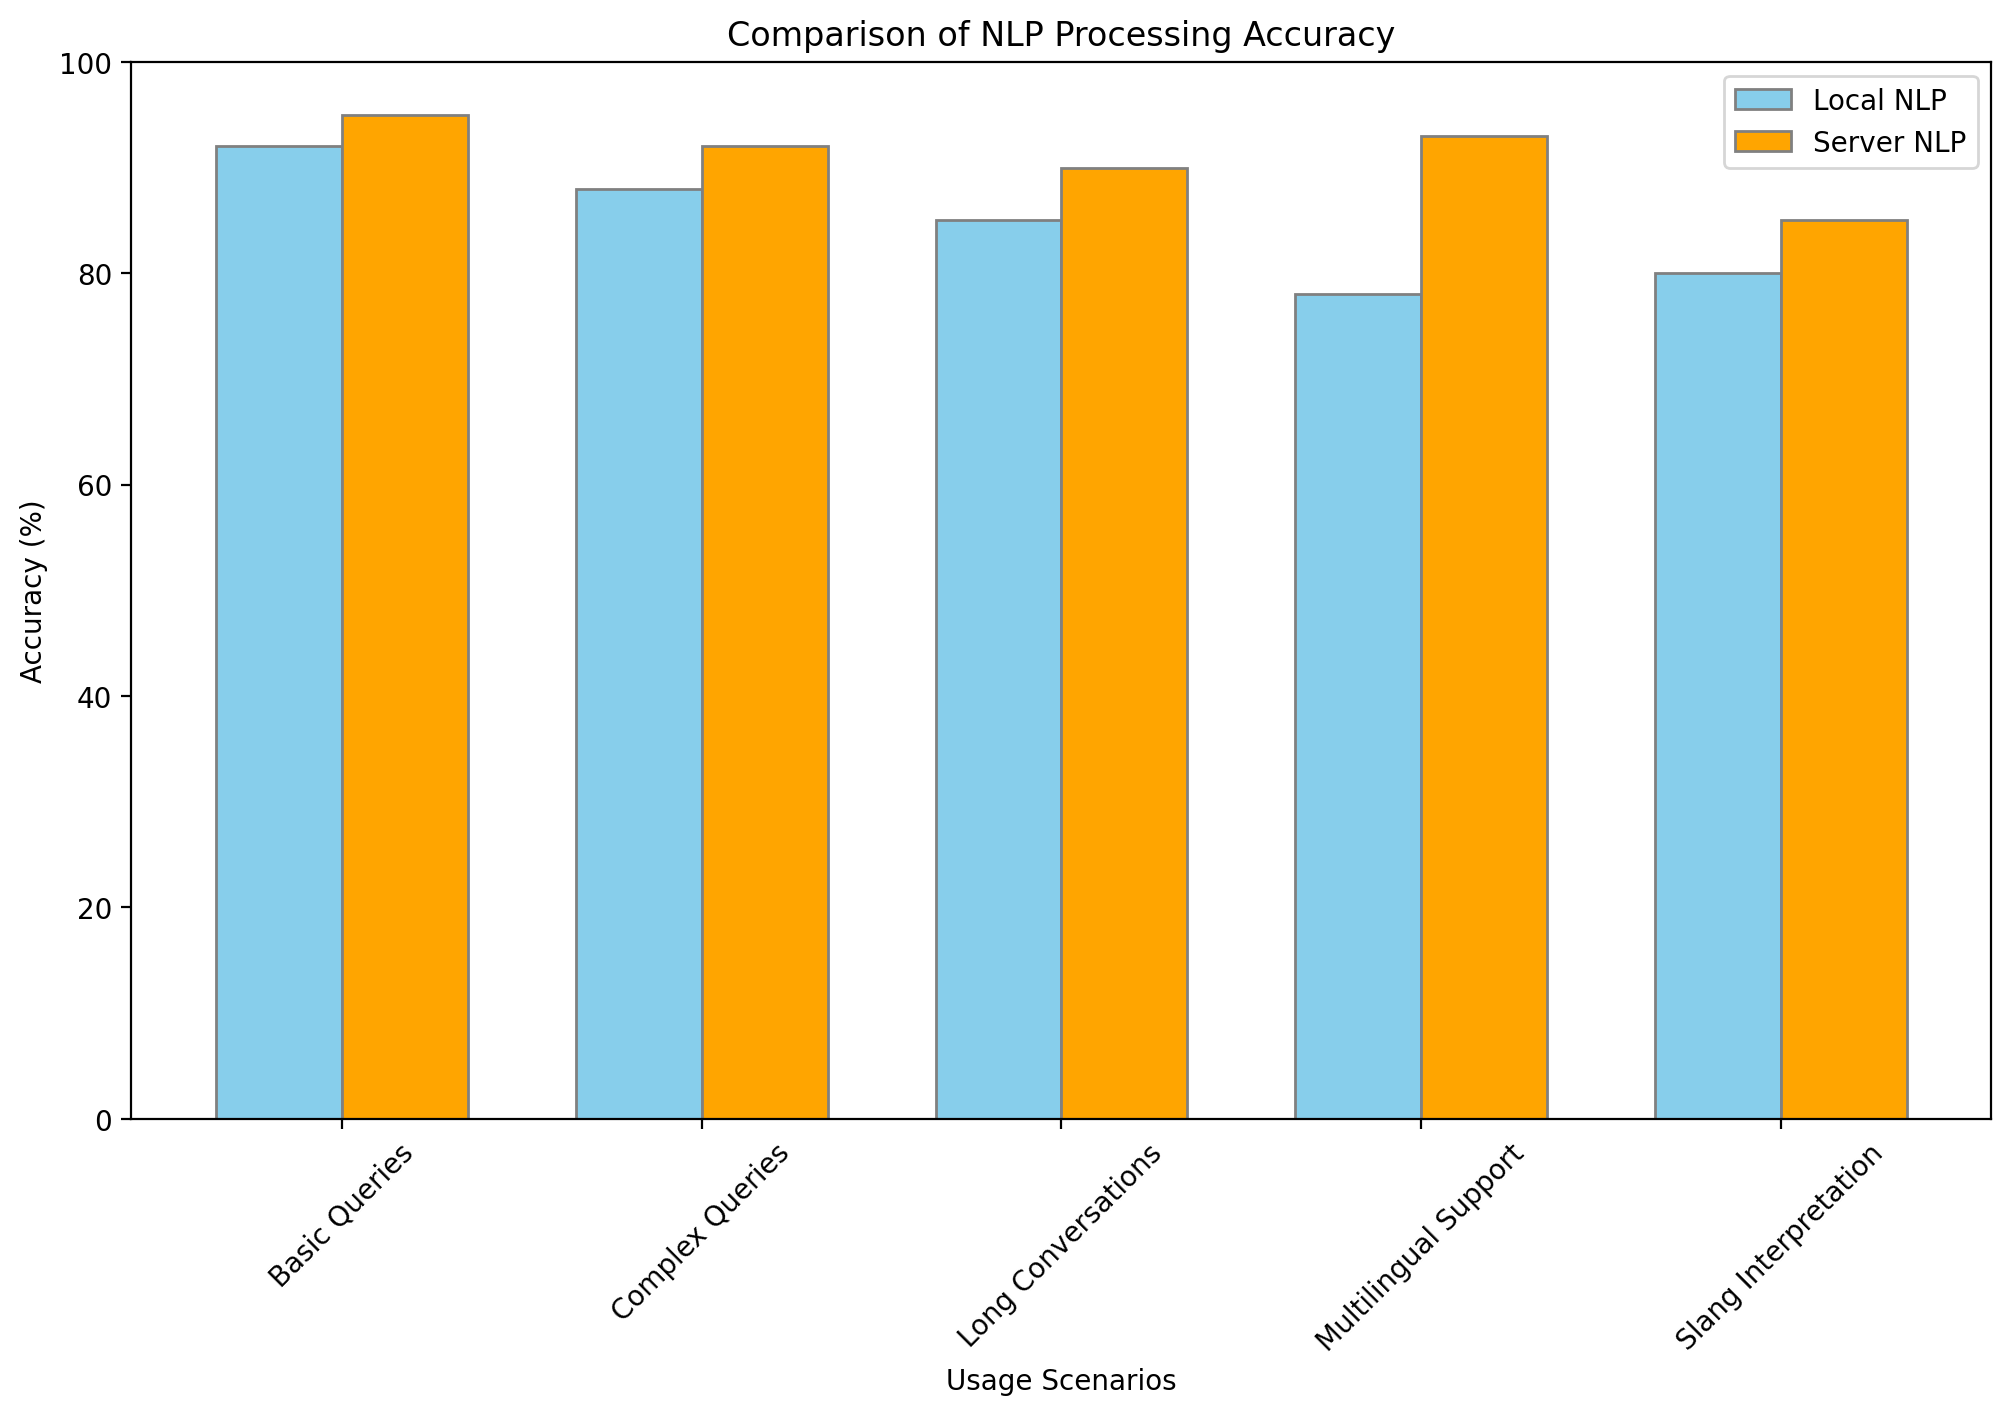
\includegraphics[width=0.8\linewidth]{nlp_correctness_graph.png}
    \caption{Mogelijke grafiek die correctheid van lokale NLP-verwerking vergelijkt met externe serverafhankelijke benaderingen. De x-as vertegenwoordigt verschillende gebruiksscenario's, terwijl de y-as de nauwkeurigheid aangeeft als een percentage.}
    \label{fig:nlp_correctness}
\end{figure}

Figuur \ref{fig:nlp_correctness} visualiseert de vermoedelijke prestatievoordelen van het privacybewuste toetsenbord in termen van NLP-verwerkingscorrectheid. De variatie in nauwkeurigheid onder verschillende scenario's biedt inzicht in de potentieel gunstige aspecten van de lokale verwerking.

\subsubsection{Gebruikersfeedback Over Pri\-va\-cy\-be\-sch\-er\-mende Functies}

\begin{figure}[ht]
    \centering
    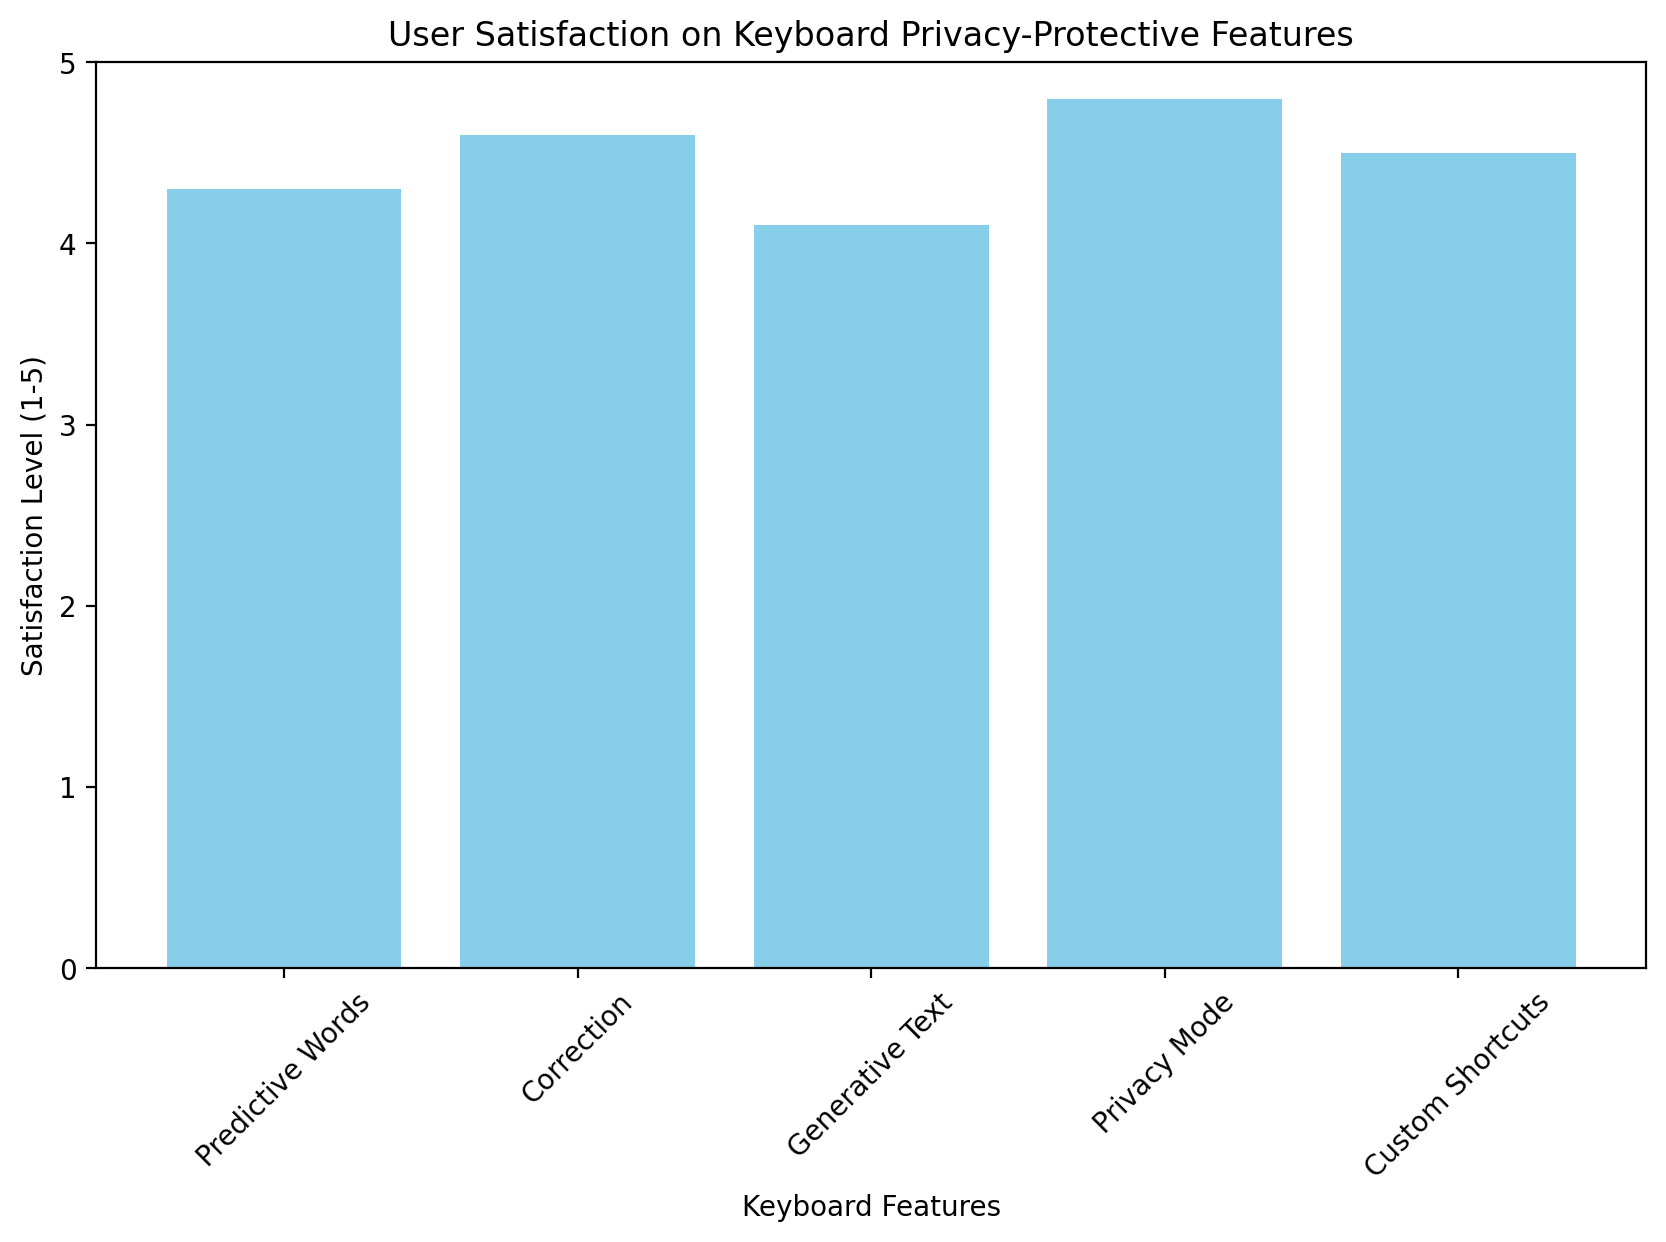
\includegraphics[width=0.8\linewidth]{user_feedback_chart.png}
    \caption{Mogelijke staafdiagram van gebruikersfeedback over toetsenbord functies. De x-as geeft verschillende functies weer, terwijl de y-as de mate van tevredenheid aangeeft op een schaal van 1 tot 5.}
    \label{fig:user_feedback}
\end{figure}

Figuur \ref{fig:user_feedback} presenteert de te verwachten reacties van gebruikers op toetsenbord functies. Door de mate van tevredenheid per functie visueel weer te geven, wordt duidelijk welke aspecten het meest gewaardeerd worden door de doelgroep.

\subsection{Conclusie}

De conclusie zal gebaseerd zijn op de vastgestelde resultaten en zal antwoord geven op de initiële onderzoeksvragen. Eventuele afwijkingen tussen de verwachte en daadwerkelijke resultaten zullen worden besproken, waarbij de impact op het vakgebied wordt belicht. Het succesvol creëren van het prototype is van cruciaal belang voor het behalen van de verwachte resultaten. Deze sectie zal de meerwaarde van de bachelorproef benadrukken door zowel technologische implementatie als gebruikerservaring in overweging te nemen.


%%---------- Andere bijlagen --------------------------------------------------
% TODO: Voeg hier eventuele andere bijlagen toe. Bv. als je deze BP voor de
% tweede keer indient, een overzicht van de verbeteringen t.o.v. het origineel.
%\input{...}

%%---------- Backmatter, referentielijst ---------------------------------------

\backmatter{}

\setlength\bibitemsep{2pt} %% Add Some space between the bibliograpy entries
\printbibliography[heading=bibintoc]

\end{document}
